%\documentclass[12pt,a4paper]{report}
%\usepackage[utf8]{inputenc}
%\usepackage{amsmath}
%\usepackage{amsfonts}
%\usepackage{amssymb}
%\usepackage[margin=2.5cm]{geometry}
%\usepackage{graphicx}
%\usepackage{caption}
%\usepackage{subcaption}
%\usepackage[nottoc,numbib]{tocbibind}
%\linespread{1.3}

%\DeclareMathOperator\sgn{sgn}

%\begin{document}
	\chapter{The Potential Step}
	\label{Potential Step}
		\begin{figure}
			\centerline{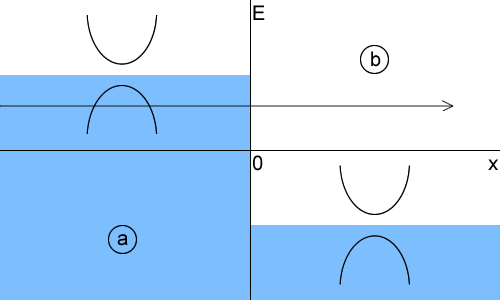
\includegraphics[scale=0.6]{images/rectangular-step-flat}}
			\caption{The graphene potential step centered at $x=0$ with potentials $|V_{a}|=|V_{b}|$ and energy gaps $m_{a,b}$ in the respective region. The parabolic dispersion relation of graphene with an energy gap has been included in each region. This case shows the possibility of Zener tunnelling as a right travelling hole becomes a left travelling electron.}
			\label{rectangular-step-flat}
		\end{figure}
		The potential step is the simplest scattering device with just two wave-function regions \cite{b13} labelled in Figure \ref{rectangular-step-flat} as $a$ and $b$, with potentials $V_{a,b}$ and energy gaps $m_{a,b}$ respectively. As well as two wave-function regions, this problem has three clear energy regions located at $E>V_{a,b}$, $|E|<|V_{a,b}|$ and $E<-V_{a,b}$. Within these regions there is pure electron transport, electron-hole transport and hole-hole transport respectively. When an energy gap is included a fourth energy region must be introduced at $E<V_{a,b}\pm m_{a,b}$ where no transport can occur. This two region problem represents a semiconductor diode and can be used to model Zener tunnelling.

%%%%%
%%%%%
%%%%%
%%%%%
%%%%%
		\section{Conservation of Probability Current}
		\label{Potential Step - Conservation of Probability Current}
			As graphene posseses a linear energy spectrum, the external potential creates an electron-hole interface at energies within the potential step. The effect of this interface is that a left travelling charge requires a left travelling electron and a right travelling hole.

			The change in charge carrier velocity causes problems with the potential step as the velocities in the initial and final region vary.  To allow for the change in velocity, the expression for the transmission probability can be checked with the current continuity equation \cite{b13, b40}:
		\begin{equation}
			\frac{d}{dt}|\psi|^{2}+\nabla\cdot \vec{j}=0
		\end{equation}
		As the system here is time independent only the probability current needs to be considered:
		\begin{equation}
			\vec{j} =\psi^{*} {\bf \sigma} \psi
		\end{equation}
		From the continuity equation, the probability current into the system must equal the probability current out of the system.
		\begin{align}
			j_{i}=j_{t}+j_{r}
			\hspace{1cm}
			1=\frac{j_{t}}{j_{i}}+\frac{j_{r}}{j_{i}}
		\end{align}
		Calculating the probability current on both sides of the step will produce the ratios of the transmitted and reflected current. Using the oscillatory wave-functions derived in Section \ref{Wave-functions - Oscillitary}, the probability current on the left of the step in the $x$ direction is:
		\begin{align}
			\psi^{*} \sigma_{x} \psi&=
			\left[\begin{array}{ccc}
				e^{-iq_{a}x}+r^{*}e^{iq_{a}x}&\alpha_{a}e^{-iq_{a}x-i\theta_{a}}-r^{*}\alpha_{a}e^{iq_{a}x+i\theta_{a}}
			\end{array}\right]
			\left[\begin{array}{ccc}
				0&1\\
				1&0
			\end{array}\right]
			\left[\begin{array}{ccc}
				e^{iq_{a}x}+re^{-iq_{a}x}\\
				\alpha_{a}e^{iq_{a}x+i\theta_{a}}-r\alpha_{a}e^{-iq_{a}x-i\theta_{a}}
			\end{array}\right]\\
			&=
			\left[\begin{array}{ccc}
				\alpha_{a}e^{-iq_{a}x-i\theta_{a}}-r^{*}\alpha_{a}e^{iq_{a}x+i\theta_{a}}&e^{-iq_{a}x}+r^{*}e^{iq_{a}x}
			\end{array}\right]
			\left[\begin{array}{ccc}
				e^{iq_{a}x}+re^{-iq_{a}x}\\
				\alpha_{a}e^{iq_{a}x+i\theta_{a}}-r\alpha_{a}e^{-iq_{a}x-i\theta_{a}}
			\end{array}\right]\\
			&=
			2\alpha_{a}\cos(\theta_{a})-2|r|^{2}\alpha_{a}\cos(\theta_{a})
		\end{align}
		On the right side of the step, the probability current becomes:
		\begin{align}
			\psi^{*} \sigma_{x} \psi&=
			\left[\begin{array}{ccc}
				t^{*}e^{-iq_{b}x}&t^{*}\alpha_{b}e^{-iq_{b}x-i\theta_{b}}
			\end{array}\right]
			\left[\begin{array}{ccc}
				0&1\\
				1&0
			\end{array}\right]
			\left[\begin{array}{ccc}
				te^{iq_{b}x}\\
				t\alpha_{b}e^{iq_{b}x+i\theta_{b}}
			\end{array}\right]\\
			&=
			2|t|^{2}\alpha_{b}\cos(\theta_{b})
		\end{align}
		Conservation of probability current requires that the current on the left of the step must be equal to the current on the right of the step. Splitting the left and right currents into the incident, reflected and transmitted components, the evaluated values for $j_{i,t,r}$ become:
		\begin{equation}
			1=|t|^{2}\frac{\alpha_{b}\cos(\theta_{b})}{\alpha_{a}\cos(\theta_{a})}+|r|^{2},
		\end{equation}
		showing that the transmission probability is given by 
		
		%showing that the normal method of using $T=|t|^{2}$ as the transmission probability does not hold for asymmetrical systems. With this modification the transmission probability can now be found by:
		\begin{equation}
			%T=1-R
			%\hspace{1cm}
			T=|t|^{2}\frac{\alpha_{b}\cos(\theta_{b})}{\alpha_{a}\cos(\theta_{a})}\cdot
			\label{newT}
		\end{equation}
		$\alpha_{b}\cos(\theta_{b})/\alpha_{a}\cos(\theta_{a})$ is the ratio of the $x$ component of the group velocities in regions $a$ and $b$. In the case where the two regions are the same, the initial and final velocities are equal and the transmission probability reduces to $T=|t|^{2}$.

			The difference in mediums inside the step also means the direction of charge carriers must be considered. For a right travelling charge an electron must travel in the right direction, however as a hole has the opposite charge, a hole must travel to the left in order for the overall charge to travel right. In this model this change in charge is represented by introducing the phase change $\theta_{h}=\pi-\theta_{e}$ \cite{b40} for wave-functions that represent hole transport. The subscript $h$ and $e$ introduced here represents the incident angles for holes and electrons respectively.
%%%%%
%%%%%
%%%%%
%%%%%
%%%%%
		\section{Simultaneous Equations}
		\label{Potential Step - Simultaneous Equations}
		The system in Figure \ref{rectangular-step-flat} can be described with the previously derived wave-functions as a set of simultaneous equations. Continuity of the wave-functions require that at the barrier interface the wave-function on the left of the step must be equal to the wave-function on the right of the step. The equation $\psi_{a}=\psi_{b}$ can be written as a set of simultaneous equations:
		\begin{align}
			e^{ik_{y}y}\left(e^{iq_{a}x}+re^{-iq_{a}x}\right)&=te^{iq_{b}x}e^{ik_{y}y}\\
			e^{ik_{y}y}\left(\alpha_{a}e^{iq_{a}x+i\theta_{a}}-r\alpha_{a}e^{-iq_{a}x-i\theta_{a}}\right)&=t\alpha_{b}e^{-iq_{b}x-i\theta_{b}}e^{ik_{y}y}
		\end{align}
		The subscripts $a$ and $b$ represent constants for the corresponding region in Figure \ref{rectangular-step-flat}. By setting the boundary between the two regions as $x=0$ these simultaneous equations will reduce to:
		\begin{align}
			1+r&=t\\
			\alpha_{a}e^{i\theta_{a}}-r\alpha_{a}e^{-i\theta_{a}}&=t\alpha_{b}e^{-i\theta_{b}}
		\end{align}
		Solving the equations for $t$ produces:
		\begin{equation}
			t=\frac{2\alpha_{a}\cos(\theta_{a})}{\alpha_{a}e^{-i\theta_{a}}+\alpha_{b}e^{i\theta_{b}}}
		\end{equation}
		The expression for $|t|^{2}$ is then:
		\begin{equation}
			|t|^{2}=\frac{4\alpha_{a}^{2}\cos^{2}(\theta_{a})}{\alpha_{a}^{2}+\alpha_{b}^{2}+2\alpha_{a}\alpha_{b}\cos(\theta_{a}+\theta_{b})}
		\end{equation}
		However, from Section \ref{Potential Step - Conservation of Probability Current}, it is known that the transmission probability through the step is not simply $T=|t|^{2}$. With Equation (\ref{newT}) the expression for the transmission probability from the conservation of current calculation becomes:
		\begin{equation}
			T=\frac{4\alpha_{a}\alpha_{b}\cos(\theta_{a})\cos(\theta_{b})}{\alpha_{a}^{2}+\alpha_{b}^{2}+2\alpha_{a}\alpha_{b}\cos(\theta_{a}+\theta_{b})}
		\end{equation}
%%%%%
%%%%%
%%%%%
%%%%%
%%%%%
		\section{Transfer and Scattering Matrices}
		\label{Potential Step - Transfer and Scattering Matrices}
		The transfer and scattering matrices can be derived for a massive potential step in graphene. When comparing the wave-functions here to that in Section \ref{Potential Step - Simultaneous Equations}, an extra reflection term must be included after the boundary in order to construct a transfer matrix. Requiring continuity at the boundary between regions $a$ and $b$ causes the wave-functions $\psi_{a}$ and $\psi_{b}$ to become equal, in matrix form this can be written as:
		\begin{align}
			e^{ik_{y}y}
			\left[\begin{array}{ccc}
				e^{iq_{a}x}&e^{-iq_{a}x}\\
				\alpha_{a}e^{iq_{a}x+i\theta_{a}}&-\alpha_{a}e^{-iq_{a}x-i\theta_{a}}
			\end{array}\right]
			\left[\begin{array}{ccc}
				a_{1}\\
				a_{2}
			\end{array}\right]
			&=
			e^{ik_{y}y}
			\left[\begin{array}{ccc}
				e^{iq_{b}x}&e^{-iq_{b}x}\\
				\alpha_{b}e^{iq_{b}x+i\theta_{b}}&-\alpha_{b}e^{-iq_{b}x-i\theta_{b}}
			\end{array}\right]
			\left[\begin{array}{ccc}
				a_{3}\\
				a_{4}
			\end{array}\right]
		\end{align}
		The subscript lettering for $q, \theta, V, m$ and $\alpha$ have been introduced to seperate constants in the corresponding step regions. Setting the boundary to $x=0$ reduces this equation to:
		\begin{align}
			\left[\begin{array}{ccc}
				1&1\\
				\alpha_{a}e^{i\theta_{a}}&-\alpha_{a}e^{-i\theta_{a}}
			\end{array}\right]
			\left[\begin{array}{ccc}
				a_{1}\\
				a_{2}
			\end{array}\right]
			&=
			\left[\begin{array}{ccc}
				1&1\\
				\alpha_{b}e^{i\theta_{b}}&-\alpha_{b}e^{-i\theta_{b}}
			\end{array}\right]
			\left[\begin{array}{ccc}
				a_{3}\\
				a_{4}
			\end{array}\right]
		\end{align}
		For simplicity we will introduce the matrices $m_{1}$ and $m_{2}$ to represent the wave-functions on each side of the step so that:
		\begin{align}
			m_{1}\left[\begin{array}{ccc}
				a_{1}\\
				a_{2}
			\end{array}\right]
			&=
			m_{2}\left[\begin{array}{ccc}
				a_{3}\\
				a_{4}
			\end{array}\right]
		\end{align}
		Then the transfer matrix $M$ can be written as:
		\begin{align}
			M&=m_{2}^{-1}m_{1}\\
			&=
			\frac{1}{2\alpha_{b}e^{-i\theta_{b}}\cos(\theta_{b})}\left[\begin{array}{ccc}
				\alpha_{b}+\alpha_{a}e^{i\theta_{a}+i\theta_{b}}&\alpha_{b}-\alpha_{a}e^{-i\theta_{a}+i\theta_{b}}\\
				\alpha_{b}e^{2i\theta_{b}}-\alpha_{a}e^{i\theta_{a}+i\theta_{b}}&\alpha_{b}e^{2i\theta_{b}}+\alpha_{a}e^{-i\theta_{a}+i\theta_{b}}
			\end{array}\right]
		\end{align}
		The scattering matrix $S$ \cite{b18} is defined as:
		\begin{align}
			S&=
			\left[\begin{array}{ccc}
				-\frac{M_{21}}{M_{22}}&\frac{1}{M_{22}}\\
				M_{11}-\frac{M_{12}M_{21}}{M_{22}}&\frac{M_{12}}{M_{22}}
			\end{array}\right]\\
			&=
			\frac{1}{\alpha_{a}+\alpha_{b}e^{i\theta_{a}+i\theta_{b}}}\left[\begin{array}{ccc}
				\alpha_{a}e^{2i\theta_{a}}-\alpha_{b}e^{i\theta_{a}+i\theta_{b}}&2\alpha_{b}e^{i\theta_{a}-2i\theta_{b}}\cos(\theta_{b})\\
				2\alpha_{a}e^{-i\theta_{a}}\cos(\theta_{a})&\alpha_{b}e^{i\theta_{a}-i\theta_{b}}-\alpha_{a}
			\end{array}\right]
		\end{align}
		With the properties:
		\begin{align}
			S_{2,2}=r\hspace{1cm}S_{1,2}=t\hspace{1cm}1=R+T\hspace{1cm}R=|r|^{2}
		\end{align}
		The modulus of $t$ is:
		\begin{equation}
			|t|^{2}=\frac{4\alpha_{b}^{2}\cos^{2}(\theta_{b})}{\alpha_{a}^{2}+\alpha_{b}^{2}+2\alpha_{a}\alpha_{b}\cos(\theta_{a}+\theta_{b})}
		\end{equation}
		This result varies from the result for $|t|^{2}$ in Section \ref{Potential Step - Simultaneous Equations}. This variation is caused by the extra reflected term added in order to create the matrices. However, as the reflection probability from the probability current is unaffected, the transmission probability can still be found by using the relation $T=1-R$. The reflection probability $R$ can be found directly from the scattering matrix:
		\begin{equation}
			r=\frac{\alpha_{b}e^{i\theta_{a}-i\theta_{b}}-\alpha_{a}}{\alpha_{a}+\alpha_{b}e^{i\theta_{a}+i\theta_{b}}}
			\hspace{1cm}
			R=|r|^{2}=\frac{\alpha_{a}^{2}+\alpha_{b}^{2}-2\alpha_{a}\alpha_{b}\cos(\theta_{a}-\theta_{b})}{\alpha_{a}^{2}+\alpha_{b}^{2}+2\alpha_{a}\alpha_{b}\cos(\theta_{a}+\theta_{b})}
			\label{stepr}
		\end{equation}
		Using this result for the reflection probability, the transmission probability through a graphene step can be found with the transfer matrix method.
		\begin{equation}
			T=1-R=\frac{4\alpha_{a}\alpha_{b}\cos(\theta_{a})\cos(\theta_{b})}{\alpha_{a}^{2}+\alpha_{b}^{2}+2\alpha_{a}\alpha_{b}\cos(\theta_{a}+\theta_{b})}
			\label{stept}
		\end{equation}
			This result agrees with the result in Section \ref{Potential Step - Simultaneous Equations} and is shown in Figure \ref{step-1} and Figure \ref{step-3}. As the expression for the transmission probability in Section \ref{Potential Step - Simultaneous Equations} agrees with the result in Equation (\ref{stept}) it is obvious that the expression for $|t|^{2}$ from the transfer matrix cannot be used to find the transmission probability. For the gap-less potential step the transmission probability will become one at all energies when the incident angle becomes zero. This property is removed if an energy gap is included, when the energy of the incident particle is within the gap region the transmission probability will become $\sim$zero. A special case for when $E=V_{a,b}$ is also present in this result for the transmission probability. When no energy gap is present the $\alpha_{a,b}$ terms will become equal to the sign function $\sgn\left(E-V_{a,b}\right)$. This sign function will cause zero transmission probability when $E=V_{a,b}$, which is often overlooked when considering graphene devices.
		\begin{figure}[h]
			 \begin{subfigure}[h]{0.5\textwidth}
				\centerline{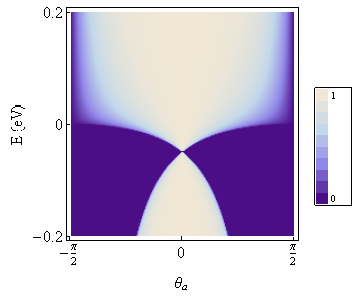
\includegraphics[scale=0.5]{images/step-1}}
				\caption{$V_{a}=0.05$ eV, $V_{b}=-0.05$ eV}
			\end{subfigure}
			\hspace{0.5cm}
			\begin{subfigure}[h]{0.5\textwidth}
				\centerline{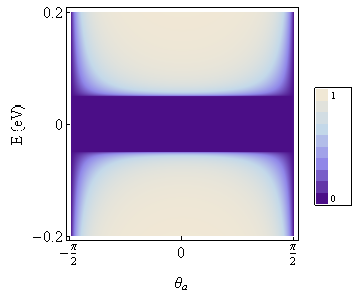
\includegraphics[scale=0.5]{images/step-2}}
				\caption{$m_{a}=0.05$ eV and $m_{b}=0$ eV}
			\end{subfigure}
			\caption{Density plots for the transmission probability against energy and incident angle for a graphene step from Equation (\ref{stept}).}
			\label{step-1}
		\end{figure}
		\begin{figure}[h]
			\begin{subfigure}[h]{0.5\textwidth}
				\centerline{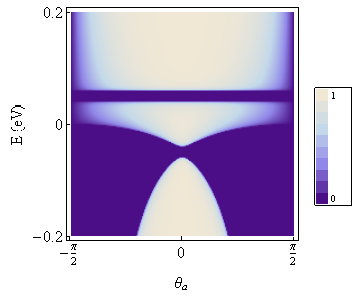
\includegraphics[scale=0.5]{images/step-3}}
				\caption{$V_{a}=0.05$ eV, $V_{b}=-0.05$ eV, $m_{a,b}=0.01$ eV}
			\end{subfigure}
			\hspace{0.5cm}
			\begin{subfigure}[h]{0.5\textwidth}
				\centerline{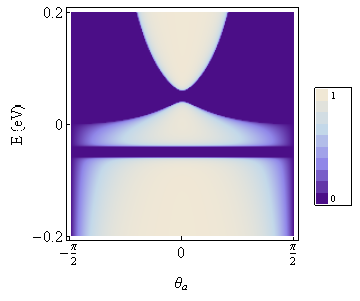
\includegraphics[scale=0.5]{images/step-4}}
				\caption{$V_{a}=-0.05$ eV, $V_{b}=0.05$ eV, $m_{a,b}=0.01$ eV}
			\end{subfigure}
			\caption{Density plots for the transmission probability against energy and incident angle for massive graphene potential step from Equation (\ref{stept}). These plots show opposing properties when the potentials are flipped.}
			\label{step-3}
		\end{figure}
%%%%%
%%%%%
%%%%%
%%%%%
%%%%%
		\section{IV Characteristics at Finite Temperatures}
		\label{Potential Step - IV Characteristics at Finite Temperatures}
			The transmission properties in Section \ref{Potential Step - Transfer and Scattering Matrices} can then be used to find the current through a scattering device. Using the Landauer formalism in Section \ref{Introduction - Landauer Formalism in Graphene} the current dependence on voltage, step height, temperature and energy gap can be obtained numerically.
			
			In Figure \ref{step-ivg-500} and Figure \ref{step-ivg-m}, current is plotted against step height. The symmetrical potential step is strongly affected by the direction of the step. When $V_{a}$ is larger than $V_{b}$ the current is overall much higher. This difference is most noticeable when the magnitude of the step is about $0.1$ eV. As expected when the direction of the step, or the external voltage is reversed the current through the step is reversed.

			When an energy gap is included the maximum value of the current is reduced. If the energy gap is present in both regions, two regions of low current will occur either side of a peak created at $V_{g}=0$. As the energy gap increases in magnitude these regions of low current will produce zero current for certain step heights. If only one step region has an energy gap, a single area of low current will occur at the step height of that step region. These effects can be seen in Figure \ref{step-ivg-m}.
		\begin{figure}[h]
			 \begin{subfigure}[h]{0.3\textwidth}
				\centerline{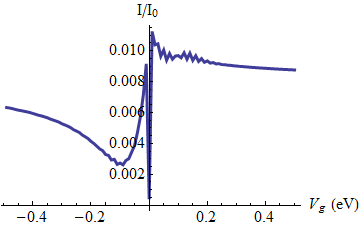
\includegraphics[scale=0.35]{images/step-vg-1}}
				\caption{$V_{sd}=0.1$ V, $V_{a}=V_{g}$ and $V_{b}=-V_{g}$.}
			\end{subfigure}
			\hspace{0.5cm}
			\begin{subfigure}[h]{0.3\textwidth}
				\centerline{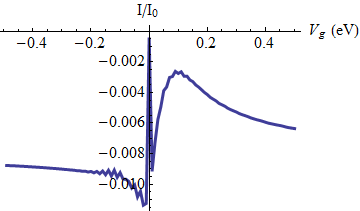
\includegraphics[scale=0.35]{images/step-vg-2}}
				\caption{$V_{sd}=-0.1$ V, $V_{a}=V_{g}$ and $V_{b}=-V_{g}$.}
			\end{subfigure}
			\hspace{0.5cm}
			\begin{subfigure}[h]{0.3\textwidth}
				\centerline{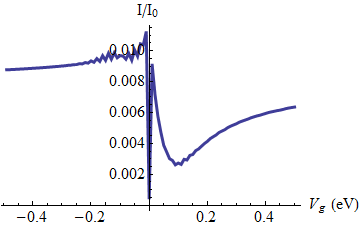
\includegraphics[scale=0.35]{images/step-vg-3}}
				\caption{$V_{sd}=0.1$ V, $V_{a}=-V_{g}$ and $V_{b}=V_{g}$.}
			\end{subfigure}
			\caption{Current against step height for symmetrical graphene potential steps from Equation (\ref{introduction-i-graphene}) with the transmission probability from Equation (\ref{stept}). For all plots $t=298$ K.}
			\label{step-ivg-500}
		\end{figure}
		\begin{figure}[h]
			 \begin{subfigure}[h]{0.3\textwidth}
				\centerline{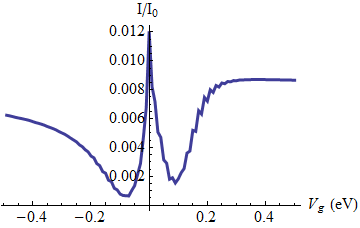
\includegraphics[scale=0.35]{images/step-vgm-1}}
				\caption{ $m_{a,b}=0.05$ eV.}
			\end{subfigure}
			\hspace{0.5cm}
			\begin{subfigure}[h]{0.3\textwidth}
				\centerline{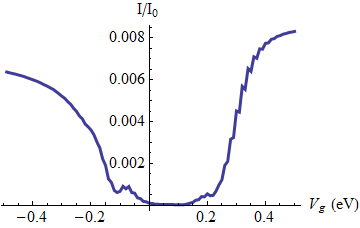
\includegraphics[scale=0.35]{images/step-vgm-2}}
				\caption{$m_{a}=0.2$ eV and $m_{b}=0$ eV.}
			\end{subfigure}
			\hspace{0.5cm}
			\begin{subfigure}[h]{0.3\textwidth}
				\centerline{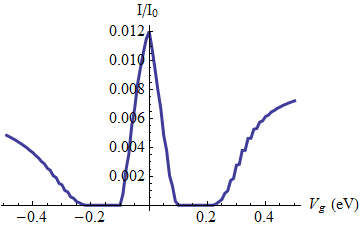
\includegraphics[scale=0.35]{images/step-vgm-3}}
				\caption{$m_{a,b}=0.2$ eV.}
			\end{subfigure}
			\caption{Current against step height for massive symmetrical graphene potential steps from Equation (\ref{introduction-i-graphene}) with the transmission probability from Equation (\ref{stept}). For all plots $V_{a}=V_{g}$, $V_{b}=-V_{g}$, $V_{sd}=0.1$ V and $t=298$ K.}
			\label{step-ivg-m}
		\end{figure}

			For a step with a fixed height the voltage across the device can be varied. Figure \ref{step-iv} shows current against source-drain voltage for a variety of graphene steps. The current through a symmetrical potential step appears to have a bias towards the positive voltages when $V_{a}>V_{b}$. This property is reversed if the step heights are reversed therefore a p-n diode is bias in the positive direction, where an n-p diode is bias in the negative direction. When an energy gap is included as in Figure \ref{step-iv} (c), the region of zero (or very low) current is expanded. Similar results were shown using the WKB method for graphene p-n junctions in \cite{b48}, relating the low current region to the voltage bias in Zener diodes and experimentaly in \cite{b57} for p-i-n diodes. 
		\begin{figure}[h]
			 \begin{subfigure}[h]{0.3\textwidth}
				\centerline{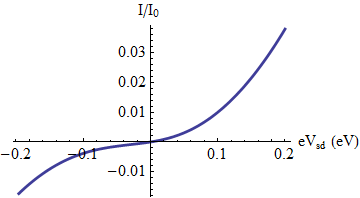
\includegraphics[scale=0.35]{images/step-v-1}}
				\caption{$V_{a}=0.05$ eV and $V_{b}=-0.05$ eV.}
			\end{subfigure}
			\hspace{0.5cm}
			\begin{subfigure}[h]{0.3\textwidth}
				\centerline{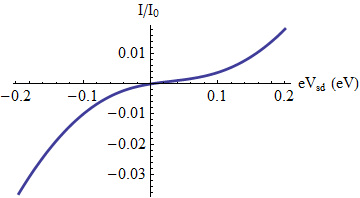
\includegraphics[scale=0.35]{images/step-v-2}}
				\caption{$V_{a}=-0.05$ eV and $V_{b}=0.05$ eV.}
			\end{subfigure}
			\hspace{0.5cm}
			\begin{subfigure}[h]{0.3\textwidth}
				\centerline{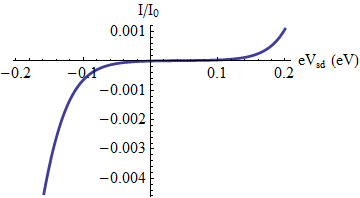
\includegraphics[scale=0.35]{images/step-v-3}}
				\caption{$V_{a}=0.05$ eV, $V_{b}=-0.05$ eV and $m_{a}=0.2$ eV.}
			\end{subfigure}
			\caption{Current against source-drain voltage for graphene potential steps from Equation (\ref{introduction-i-graphene}) with the transmission probability from Equation (\ref{stept}). For all plots $t=298$ K.}
			\label{step-iv}
		\end{figure}

			The temperature dependence on current for graphene steps is then shown in Figure \ref{step-it}. The direction of the step again contributes largely to the current at low temperatures. The current is over double when $V_{a}>V_{b}$, however, the current through the step appears to become fairly linear at higher temperatures, reducing the effect voltage and step direction has on the current. The addition of an energy gap lowers the overall current, this effect is most obvious at low temperatures. A large energy gap can reduce the current to essentially zero at lower temperatures until the linear nature of the temperature dependence re-emerges at high temperatures.
		\begin{figure}[h]
			 \begin{subfigure}[h]{0.3\textwidth}
				\centerline{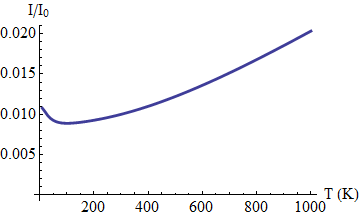
\includegraphics[scale=0.35]{images/step-t-1}}
				\caption{$V_{a}=0.05$ eV and $V_{b}=-0.05$ eV.}
			\end{subfigure}
			\hspace{0.5cm}
			\begin{subfigure}[h]{0.3\textwidth}
				\centerline{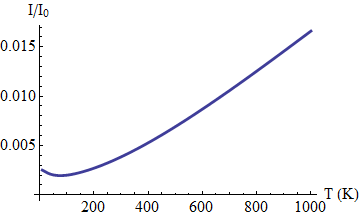
\includegraphics[scale=0.35]{images/step-t-3}}
				\caption{$V_{a}=-0.05$ eV and $V_{b}=0.05$ eV.}
			\end{subfigure}
			\hspace{0.5cm}
			\begin{subfigure}[h]{0.3\textwidth}
				\centerline{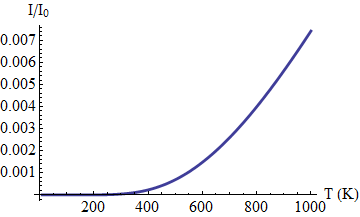
\includegraphics[scale=0.35]{images/step-t-2}}
				\caption{$V_{a}=0.05$ eV, $V_{b}=-0.05$ eV and $m_{a}=0.2$ eV.}
			\end{subfigure}
			\caption{Current against temperature for graphene potential steps from Equation (\ref{introduction-i-graphene}) with the transmission probability from Equation (\ref{stept}). For all plots $V_{sd}=0.1$ V.}
			\label{step-it}
		\end{figure}
%%%%%
%%%%%
%%%%%
%%%%%
%%%%%
		\section{Conductance}
		\label{Potential Step - Conductance}
			Following on from the current, the conductance of a sample can also be obtained. The non-infinite, zero temperature conductance formula was discussed in Section \ref{Introduction - Landauer Formalism in Graphene}. The numerical plots for zero temperature conductance with small source-drain voltages is shown in Figure \ref{step-g} for various graphene steps.
				
			At energies outside of the step the conductance follows a very linear dependence on energy. This is caused by the inclusion of the $|E_{f}|$ term from the graphene density of states. Inside the step the conductance increases away from zero and lowest step height. When the Fermi energy is equal to zero or the lowest step height the conductance reduces to zero. The conductance is also reduced to zero if an energy gap is included; the region of zero conductance is equivalent to the magnitude of the energy gap.
		\begin{figure}[h]
			 \begin{subfigure}[h]{0.3\textwidth}
				\centerline{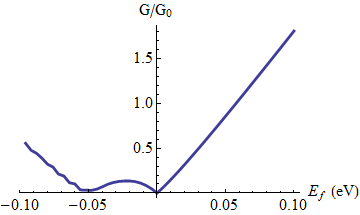
\includegraphics[scale=0.35]{images/step-g-1}}
				\caption{$V_{a}=0.05$ eV and $V_{b}=-0.05$ eV.}
			\end{subfigure}
			\hspace{0.5cm}
			\begin{subfigure}[h]{0.3\textwidth}
				\centerline{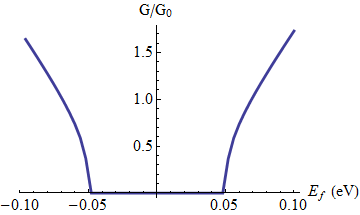
\includegraphics[scale=0.35]{images/step-g-2}}
				\caption{$m_{a}=0.05$ eV and $m_{b}=0$ eV.}
			\end{subfigure}
			\hspace{0.5cm}
			\begin{subfigure}[h]{0.3\textwidth}
				\centerline{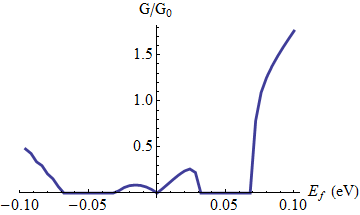
\includegraphics[scale=0.35]{images/step-g-3}}
				\caption{$V_{a}=0.05$ eV, $V_{b}=-0.05$ eV and $m_{a,b}=0.2$ eV.}
			\end{subfigure}
			\caption{The zero temperature conductance with small source-drain voltages has been plotted against Fermi energy for various graphene steps. The conductance is taken from Equation (\ref{introduction-g-zero}) with the step transmission probability from Equation (\ref{stept}).} 
			\label{step-g}
		\end{figure}
%\end{document}